\documentclass[12pt, a4paper]{article}

% --- PAQUETES ESENCIALES (Codificación, Idioma) ---
\usepackage[utf8]{inputenc}
\usepackage[spanish,es-lcroman]{babel}

% --- PAQUETES PARA CITAS Y BIBLIOGRAFÍA (MUY IMPORTANTE EL ORDEN) ---
\usepackage{csquotes}
\usepackage[
    backend=biber,
    style=apa,
    sortcites=true,
    maxcitenames=2,
    giveninits=true,
    uniquename=init,
    uniquelist=minyear,
    maxbibnames=99,
    date=year,
    urldate=long,
    isbn=false,
    doi=true,
    eprint=false,
    hyperref=true,
    backref=false,
    parentracker=true,
    dashed=false,
    block=space
]{biblatex}
\addbibresource{referencias.bib}

% --- PAQUETES PARA DISEÑO, FORMATO Y CONTENIDO ---
\usepackage{geometry}
\geometry{a4paper, margin=2.54cm}
\usepackage{fancyhdr}
\usepackage{tabularx}
\usepackage{booktabs}
\usepackage{float}
\usepackage{caption}
\usepackage{listings}
\usepackage{enumitem}
\usepackage{amsmath}
\usepackage{xcolor}
\usepackage{setspace}
\usepackage{mathpazo} % Para la fuente Palatino
\usepackage{graphicx}

% --- PAQUETE HYPERREF (DEBE SER DE LOS ÚLTIMOS EN CARGARSE) ---
\usepackage{xurl} % Permite saltos de línea en URLs
\usepackage{hyperref}

% --- CONFIGURACIONES DE PAQUETES (DESPUÉS DE CARGARLOS) ---
\hypersetup{
    colorlinks=true,
    linkcolor=blue!50!black,
    citecolor=blue!50!black,
    urlcolor=cyan!50!black,
    pdftitle={Informe de Diagramas de Procesos Organizacionales para un Sistema de Gemelo Digital de Mantenimiento},
    pdfauthor={Juan David Julio Serrano}
}

\newcolumntype{L}{>{\raggedright\arraybackslash}X} 

\definecolor{codegray}{rgb}{0.5,0.5,0.5}
\lstset{
    basicstyle=\ttfamily\small, breaklines=true, frame=single,
    showstringspaces=false, numbers=left, numberstyle=\tiny\color{codegray},
    keywordstyle=\color{blue},
    commentstyle=\color{green!40!black},
    stringstyle=\color{purple}
}

\captionsetup{
    format=plain,
    labelfont=bf,
    textfont=normalfont,
    singlelinecheck=false,
    justification=centering
}

% ===================================================================
%                       METADATOS DEL DOCUMENTO
% ===================================================================
\title{Informe de Diagramas de Procesos Organizacionales para un Sistema de Gemelo Digital de Mantenimiento}
\author{Juan David Julio Serrano}
\date{14 de noviembre de 2025}

% ===================================================================
%                       INICIO DEL DOCUMENTO
% ===================================================================
\begin{document}

% --- PORTADA ---
\begin{titlepage}
    \begin{center}
        \vspace*{2.5cm}
        {\Huge \bfseries Informe de Diagramas de Procesos Organizacionales para un Sistema de Gemelo Digital de Mantenimiento}\\[2cm]
        
        {\large \bfseries Aprendices:}\\[0.5cm]
        \large{Juan David Julio Serrano (Ficha: 3336237)}\\[0.3cm]
        \large{Maria Juliana Calvo Corredor (Ficha: 3336237)}\\[0.3cm]
        \large{Jesús David Algeciras Abril (Ficha: 3336238)}\\[0.3cm]
        \large{Didier Moreno Caicedo (Ficha: 3336238)}\\[1.2cm]
        
        {\large \bfseries Instructor:}\\[0.5cm]
        \large{Ing. Wilson Alberto Mosquera Caicedo}\\[1.5cm]
        
        \vspace{1cm}
        \large{Servicio Nacional de Aprendizaje (SENA)}\\[0.4cm]
        \large{Centro de Biotecnología Industrial - Regional Valle}\\[0.4cm]
        \large{Tecnología en Análisis y Desarrollo de Software (ADSO)}\\[1.2cm]
        \large{14 de noviembre de 2025}
    \end{center}
\end{titlepage}

\doublespacing

% --- CONTENIDO DEL DOCUMENTO ---
\section{Introducción}

El presente documento complementa el análisis de procesos organizacionales previo mediante una esquematización visual de los flujos de trabajo clave del \textbf{Sistema de Gemelo Digital para Mantenimiento}. El objetivo de este mapa de procesos es traducir los requisitos funcionales en una secuencia lógica de actividades, decisiones y responsabilidades, proporcionando una visión clara y unificada de cómo operará el software.

Para la modelación de los procesos, se ha utilizado el estándar \textbf{BPMN 2.0 (Business Process Model and Notation)}, una notación gráfica mantenida por el Object Management Group (OMG) \parencite{omg:2013}. Esta notación fue seleccionada por su capacidad para servir como un lenguaje común, permitiendo que tanto los perfiles técnicos (desarrolladores, arquitectos) como los de negocio y gestión (supervisores, gerentes) comprendan de manera inequívoca el funcionamiento del sistema, facilitando así la validación, el diseño y la futura implementación del proyecto.

\section{Descripción del Proceso: Ciclo de Mantenimiento Correctivo}

El siguiente diagrama BPMN modela el flujo de trabajo para el \textbf{Ciclo de Mantenimiento Correctivo}. Este proceso se activa de manera reactiva, es decir, cuando se detecta una anomalía o un fallo en un activo durante la operación normal. Su objetivo es restaurar la funcionalidad del equipo de la manera más eficiente posible, asegurando al mismo tiempo una correcta documentación para el análisis histórico.

\begin{figure}[H]
    \centering
    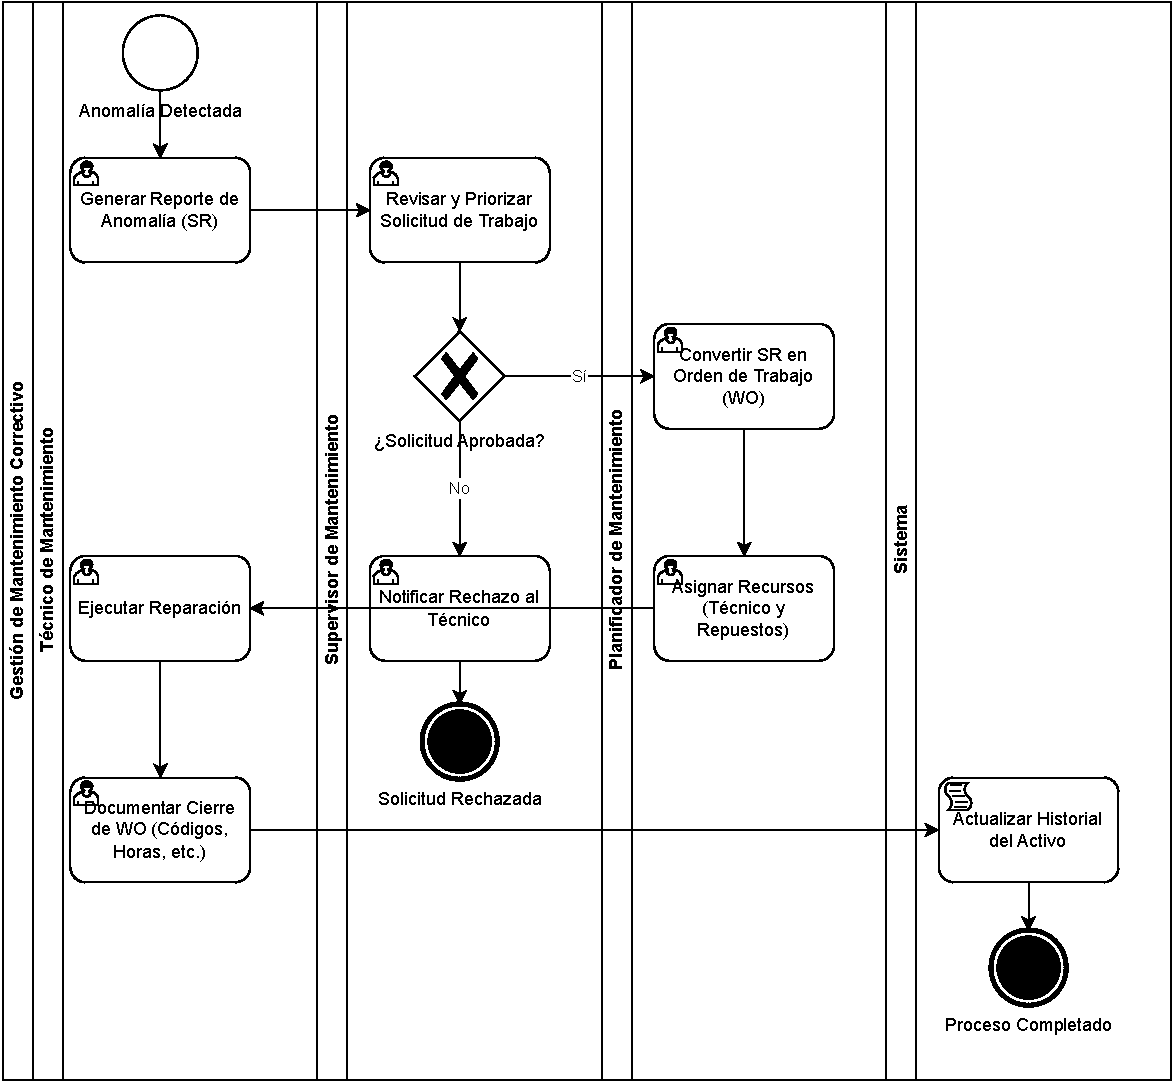
\includegraphics[width=\textwidth]{Imagenes/Diagrama_BPMN_CM.pdf}
    \caption{Diagrama BPMN del Ciclo de Mantenimiento Correctivo.}
\end{figure}

El proceso se compone de cuatro carriles (\textit{lanes}) principales que representan a los actores y sistemas participantes: el Técnico de Mantenimiento, el Supervisor de Mantenimiento, el Planificador de Mantenimiento y el Sistema de software.

El flujo de trabajo se desarrolla de la siguiente manera:

\begin{enumerate}
    \item \textbf{Inicio: Anomalía Detectada.} El proceso comienza en el carril del \textbf{Técnico}, cuando este identifica una anomalía durante una inspección de rutina o recibe una notificación de un fallo operativo. Este evento sirve como disparador (\textit{Start Event}).
    \item \textbf{Generación de Reporte de Anomalía (SR):} El \textbf{Técnico} utiliza su dispositivo móvil (tablet) para crear una Solicitud de Trabajo (\textit{Service Request} o SR). En esta tarea, documenta el problema, adjunta evidencia fotográfica y clasifica la urgencia inicial.
    \item \textbf{Revisión y Priorización:} La SR llega al carril del \textbf{Supervisor}, quien es responsable de analizar la solicitud. En esta tarea, evalúa el impacto del fallo en la operación y determina su prioridad.
    \item \textbf{Decisión de Aprobación:} El flujo alcanza una compuerta de decisión (\textit{Exclusive Gateway}), donde el \textbf{Supervisor} evalúa si la solicitud es válida y requiere acción inmediata.
    \begin{itemize}
        \item \textbf{Si la solicitud es rechazada (No)}, el Supervisor ejecuta la tarea de Notificar Rechazo al Técnico, documentando la razón (ej. ``falsa alarma'', ``duplicado''). El proceso finaliza en este punto (\textit{End Event}).
        \item \textbf{Si la solicitud es aprobada (Sí)}, el flujo continúa.
    \end{itemize}
    \item \textbf{Conversión a Orden de Trabajo (WO):} El \textbf{Supervisor} convierte la solicitud (SR) en una Orden de Trabajo (WO) formal, asignándole un número de seguimiento y validando la información.
    \item \textbf{Asignación de Recursos:} La WO pasa al carril del \textbf{Planificador}, quien se encarga de la logística. En esta tarea, verifica la disponibilidad de personal, asigna al técnico más adecuado y reserva los repuestos y herramientas necesarios del inventario (MRO).
    \item \textbf{Ejecución de la Reparación:} La WO, ya con todos los recursos asignados, vuelve al carril del \textbf{Técnico}. Este ejecuta el trabajo físico de reparación en la planta, siguiendo las instrucciones de la orden.
    \item \textbf{Documentación de Cierre:} Una vez finalizada la reparación, el \textbf{Técnico} realiza una tarea fundamental para el sistema: la documentación del cierre de la WO. En esta etapa, registra datos estructurados como las horas-hombre utilizadas, los repuestos consumidos, los códigos de causa de la falla y una descripción de la solución aplicada.
    \item \textbf{Actualización del Historial:} La información de cierre es procesada automáticamente en el carril del \textbf{Sistema}. El software actualiza de forma permanente el historial de mantenimiento del activo, alimentando la base de datos que será utilizada para futuros análisis de KPIs como el MTTR y el MTBF.
    \item \textbf{Fin del Proceso:} Con el historial actualizado, el ciclo de mantenimiento correctivo se da por finalizado (\textit{End Event}).
\end{enumerate}

\section{Descripción del Proceso: Ciclo de Mantenimiento Preventivo (PM)}

El siguiente diagrama BPMN modela el flujo de trabajo para el \textbf{Ciclo de Mantenimiento Preventivo (PM)}. Este proceso se activa de manera proactiva, basándose en un plan de mantenimiento predefinido por tiempo o uso. Su objetivo es ejecutar tareas programadas para anticipar fallos, maximizar la vida útil de los activos y asegurar una correcta documentación para el análisis histórico y la mejora continua.

\begin{figure}[H]
    \centering
    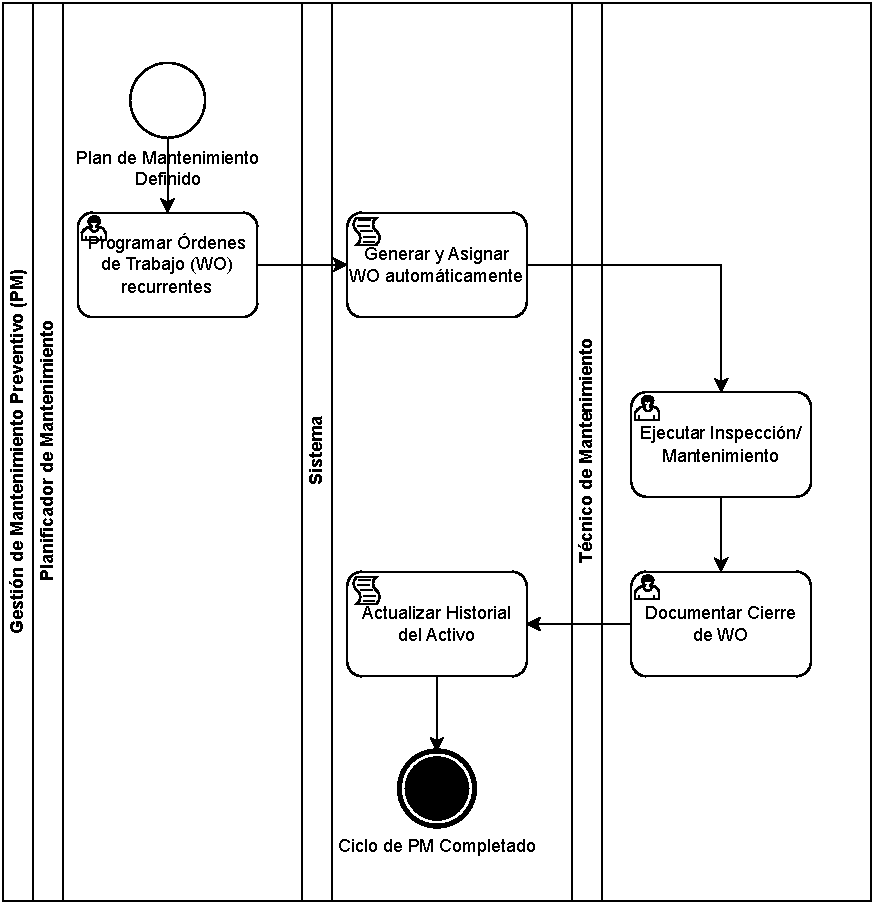
\includegraphics[width=\textwidth]{Imagenes/Diagrama_BPMN_PM.pdf}
    \caption{Diagrama BPMN del Ciclo de Mantenimiento Preventivo.}
\end{figure}

El flujo involucra a tres carriles (\textit{lanes}) principales: el Planificador de Mantenimiento, el Sistema de software y el Técnico de Mantenimiento.

El flujo de trabajo se desarrolla de la siguiente manera:

\begin{enumerate}
    \item \textbf{Inicio: Planificación.} El proceso se inicia en el carril del \textbf{Planificador de Mantenimiento}, quien, basándose en un Plan de Mantenimiento Definido (\textit{Start Event}), realiza la tarea de Programar Órdenes de Trabajo (WO) recurrentes. En este paso, configura en el sistema las tareas periódicas (ej. ``inspección trimestral'', ``lubricación cada 500 horas de uso'').
    \item \textbf{Generación Automática:} La responsabilidad se transfiere al carril del \textbf{Sistema}. Basado en la programación establecida (por fecha o umbral de uso), el software ejecuta la tarea de Generar y Asignar WO automáticamente. Esto crea una nueva orden de trabajo con todos los detalles necesarios y la asigna al técnico correspondiente, notificándole en su dispositivo. A diferencia del ciclo de mantenimiento correctivo, este flujo no requiere una aprobación explícita del Supervisor para cada orden de trabajo, ya que la tarea se origina a partir de un plan de mantenimiento previamente autorizado.
    \item \textbf{Ejecución en Campo:} La orden de trabajo aparece en la lista de tareas del \textbf{Técnico de Mantenimiento}. Este se desplaza al activo y procede a Ejecutar Inspección/Mantenimiento, realizando la labor física en la planta siguiendo la lista de verificación y los procedimientos definidos en la WO.
    \item \textbf{Documentación de Cierre:} Una vez completado el trabajo, el \textbf{Técnico} realiza la tarea de Documentar Cierre de WO, registrando la finalización de la tarea, las observaciones pertinentes y cualquier material utilizado. Este paso es crucial para la trazabilidad.
    \item \textbf{Actualización del Sistema:} La información del cierre es enviada de vuelta al carril del \textbf{Sistema}, el cual ejecuta la tarea final de Actualizar Historial del Activo, añadiendo un nuevo registro al historial del equipo.
    \item \textbf{Fin del Proceso:} Con el historial actualizado, el ciclo de mantenimiento preventivo se da por finalizado (Ciclo de PM Completado).
\end{enumerate}

\section{Descripción del Proceso: Ciclo de Mantenimiento Predictivo (PdM)}

El siguiente diagrama BPMN modela el flujo de trabajo para el \textbf{Ciclo de Mantenimiento Predictivo (PdM)}. Este proceso representa la estrategia más avanzada de gestión de activos, donde el objetivo es pasar de reaccionar a fallos a \textbf{pronosticarlos y prevenirlos}. Se basa en la monitorización continua del estado real del equipo y la aplicación de modelos de inteligencia artificial para tomar decisiones proactivas.

\begin{figure}[H]
    \centering
    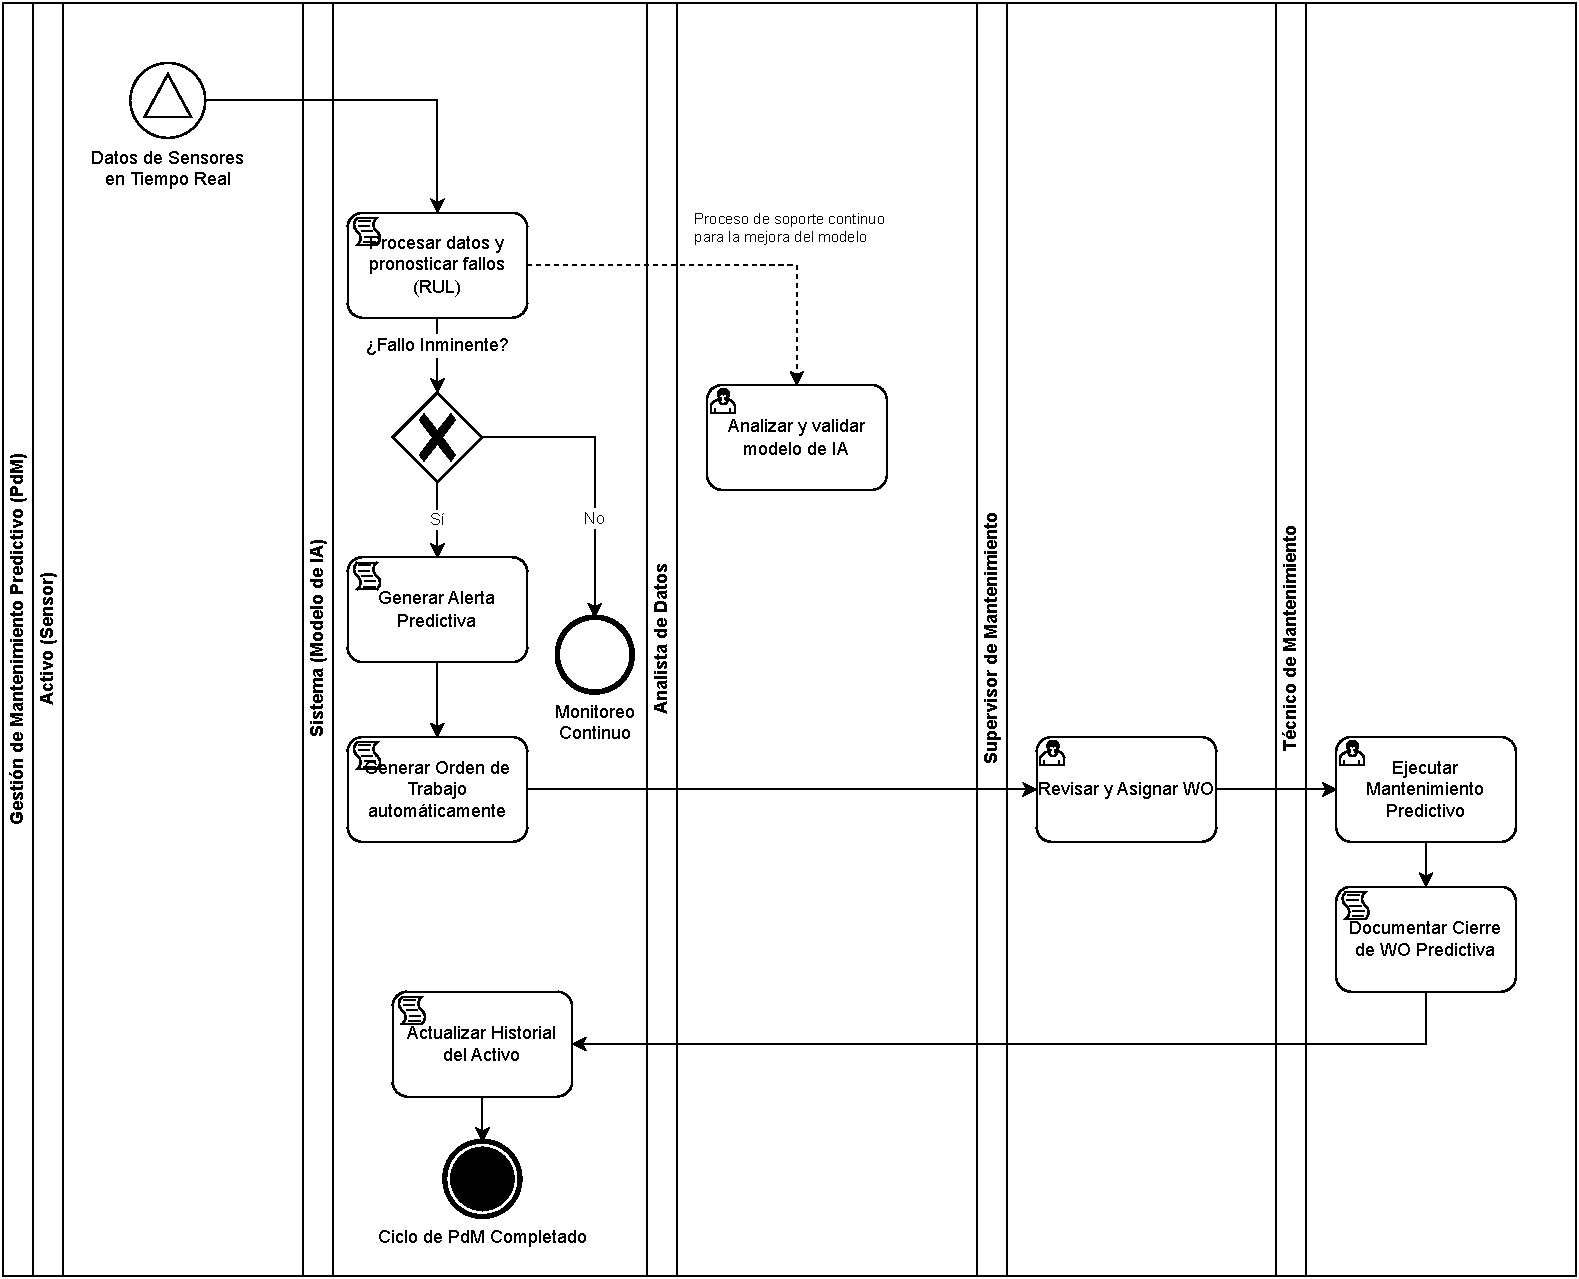
\includegraphics[width=\textwidth]{Imagenes/Diagrama_BPMN_PdM.pdf}
    \caption{Diagrama BPMN del Ciclo de Mantenimiento Predictivo.}
\end{figure}

El flujo involucra a cuatro carriles (\textit{lanes}) que representan la interacción entre el mundo físico y el digital: el Activo (Sensor), el Sistema (Modelo de IA), el Analista de Datos y el Supervisor de Mantenimiento.

El flujo de trabajo se desarrolla de la siguiente manera:

\begin{enumerate}
    \item \textbf{Inicio: Monitorización Continua.} El proceso se inicia en el carril del \textbf{Activo}, con la captura constante de Datos de Sensores en Tiempo Real (\textit{Start Event}). Estos datos de entrada (vibración, temperatura, etc.) constituyen la base para el modelo predictivo.
    \item \textbf{Procesamiento y Pronóstico:} Los datos son enviados al carril del \textbf{Sistema}, donde el modelo de IA ejecuta la tarea Procesar datos y pronosticar fallos. En esta fase se calculan indicadores clave como la vida útil restante (RUL, del inglés \textit{Remaining Useful Life}) de un componente.
    \item \textbf{Decisión Predictiva:} El flujo llega a una compuerta de decisión (\textit{Exclusive Gateway}) que evalúa el resultado del modelo: ¿Fallo Inminente?.
    \begin{itemize}
        \item \textbf{Si el riesgo de fallo no es inminente (No)}, el sistema vuelve a un estado de Monitoreo Continuo (\textit{End Event}), cerrando el ciclo hasta la próxima evaluación.
        \item \textbf{Si el riesgo de fallo es alto (Sí)}, el flujo continúa hacia la acción proactiva.
    \end{itemize}
    \item \textbf{Generación de Alerta:} El \textbf{Sistema} ejecuta la tarea Generar Alerta Predictiva, notificando automáticamente a los roles pertinentes (Supervisor, Analista) sobre el riesgo detectado y el activo afectado.
    \item \textbf{Generación Automática de Orden de Trabajo:} Inmediatamente después, el \textbf{Sistema} crea una Orden de Trabajo automáticamente. Esta WO es de tipo ``Predictivo'' y contiene toda la información del pronóstico para guiar al equipo de mantenimiento.
    \item \textbf{Revisión y Asignación Humana:} La orden de trabajo generada se envía al carril del \textbf{Supervisor de Mantenimiento}. En la tarea Revisar y Asignar WO, el supervisor valida la recomendación del sistema, confirma la urgencia y la asigna formalmente a un técnico para su ejecución.
    \item \textbf{Fin del Proceso (Inicio de Mantenimiento):} Una vez asignada la WO, el ciclo predictivo concluye (con un evento de \textit{Mantenimiento Programado}) y da inicio a un flujo de ejecución similar al del mantenimiento correctivo.
\end{enumerate}

Paralelamente a este flujo operativo, el \textbf{Analista de Datos} ejerce un rol de supervisión continua. Su función es ejecutar la tarea de analizar y validar el modelo de IA, con el fin de asegurar la precisión de los pronósticos y reentrenar los modelos a medida que se recopilan más datos históricos.

% --- BIBLIOGRAFÍA ---
\clearpage
\printbibliography[heading=bibintoc,title=Referencias]

\end{document}